\documentclass[a4paper, 11pt]{article}
\usepackage[czech]{babel}
\usepackage[utf8]{inputenc}
\usepackage[IL2]{fontenc}
\usepackage{times}
\usepackage{hyperref}
\hypersetup{colorlinks=true, linkcolor=black, urlcolor=blue}
\usepackage[left=1.5cm,text={18cm, 25cm},top=2.5cm]{geometry}
\usepackage{graphicx}
\graphicspath{ {images/} }
\newcommand{\myuv}[1]{\quotedblbase #1\textquotedblleft}

\begin{document}
\begin{titlepage}
\begin{center}
	
	\textsc{\Huge Fakulta informačních technologií\\[3.5mm]
			Vysoké učení technické v~Brně}
	\\[79mm]
	{\LARGE IPK \,--\, Počítačové komunikace a sítě\\[1.5mm]
	Projekt č.1 - Zjištění informací o uživateli}
	\vfill
\end{center}
{\Large 12.3.2018 \hfill Tomáš Nereča(xnerec00)}
\\[-4mm]
\end{titlepage}
\tableofcontents
\thispagestyle{empty}
\newpage

\section{Zadanie}
Zoznámiť sa s kostrami kódov pre programovanie sieťových aplikácií (klient, server) za použitia \emph{BSD socketov}. Navrhnúť vlastný aplikačný protokol realizujúci prenos informácií o použivateľoch a naprogramovať klientskú a serverovú aplikáciu.

\section{Základné informácie}
Komunikáciu medzi serverom a klientom zabezpečuje protokol \emph{TCP}, nakoľko bolo potrebné zabezpečiť bezpečný prenos informácií bez poškodenia dát. TCP komunikácia zahŕňa nadviazanie spojenia. Pri nadväzovaní spojenia prebehne tzv. \emph{three-way handshake}. Ak je všetko v poriadku, začnú sa odosielať dáta medzi klientom a serverom. Na základe zadaných vstupných argumentov pri spúšťaní klienta sa vytvorí správa - \emph{request}, ktorá je odoslaná na server. Server následne v súbore \textbf{etc/passwd} vyhľadá požadované údaje a odošle správu obsahujúcu tieto údaje klientovi, prípadne prázdnu správu ak sa údaje nepodarilo nájsť.

\section{Popis riešenia}

\subsection{Klient}
Kontrolu vstupných argumentov v oboch aplikáciách zabezpečuje funkcia \textsc{getopt()}. V prípade nesprávnej kombinácie, prípadne chýbajúcich argumentov aplikácia vypíše nápovedu a skončí.

Po kontrole argumentov sa vytvorí request, ktorý obsahuje hlavičku v tvare \verb|<--xnerec00_protocol-->|. Ďalej obsahuje číselný kód zvoleného argumentu(1, 2 alebo 3) a prípadne \textbf{login}. Jednotlivé časti sú oddelené znakom~\textbf{\&}.

Následne sa klient pokúsi nadviazať TCP komunikáciu so serverom a odoslať request. K tomu je potrebné vykonať nasledujúce kroky:

\begin{itemize}
\item vytvoriť \emph{client socket} pomocou funkcie \textsc{socket()}
\item vyhladať \emph{DNS} serveru a preložiť, prípadne skontrolovať prítomnosť serveru na zadanej \emph{IPv4} adrese pomocou funkcie \textsc{gethostbyname()}
\item pripojiť sa na server pomocou funkcie \textsc{connect()}
\item odoslať request pomocou funkcie \textsc{send()}
\end{itemize}

Po úspešnom vykonaní týchto krokov je klient pripravený príjimať dáta zo serveru. Dáta su ukladané do \emph{bufferu}. Prijatá správa je ihneď vytlačená na štandardný výstup. Prijímanie dát zabezpečuje funkcia \textsc{recv()} vo \textsc{while} cykle. Ak prijaté dáta nenaplnia buffer, signalizuje to, že server už odoslal všetky dáta. Po vyskočení z cyklu sa uzavrie client socket pomocou funkcie \textsc{close()} a aplikácia sa ukončí.

\subsection{Server}
Po validácii \textsc{portu} bude server čakať na request. K tomu je potrebné vykonať nasledujúce kroky:

\begin{itemize}
	\item vytvoriť \emph{welcome socket} pomocou funkcie \textsc{socket()}
	\item priradiť adresu k welcome socketu pomocou funkcie \textsc{bind()}
	\item pomocou funkcie \textsc{listen()} označiť welcome socket ako pasívny (bude použitý na akceptovanie requestu)
\end{itemize}

Server teraz v nekonečnom cykle čaká na request. Funkcia \textsc{accept()} pri nadviazaní spojenia vytvorí \emph{komunikačný socket} a prijme request pomocou funkcie \textsc{recv()}.

Po rozparsovaní requestu sa vytvorí správa, ktorá bude odoslaná klientovi. Request musí obsahovať správnu hlavičku. Správa bude odosielaná vo \textsc{while} cykle po bufferoch veľkosti 1024B. Po odoslaní celej správy sa komunikačný socket uzavrie a server čaká na ďalší request.

Server vybavuje requesty až do prijatia signálu \textsc{SIGINT}. Po jeho odchytení sa uzavrie welcome socket a aplikácia sa ukončí.

\section{Zaujímavosti}
Pri argumente -p prebieha ihneď kontrola, či bol zadaný validný port pomocou funkcie \textsc{find\_first\_not\_of()}.

Ak pri argumente -h je prvý znak číslo, kontroluje sa, či bola zadaná korektná IPv4 adresa pomocou funkcie \textsc{inet\_pton()}.

Client socket má nastavený timeout na 10s pomocou funkcie \textsc{setsockopt()}) s parametrom \textsc{SO\_RCVTIMEO}. Ak po uplynutí 10s nepríde odpoveď zo serveru, aplikácia sa ukončí.

Aby nedochádzalo k problému, že ihneď po vypnutí serveru sa nedá spustiť server na rovnakom porte, je po vytvorení welcome socketu zavolaná funkcia \textsc{setsockopt()}) s parametrom \textsc{SO\_REUSEADDR}. Tým pádom sa povolí re-bindovanie na port, ktorý bol použitý predtým.

Vyhľadávanie v súbore \textbf{etc/passwd} a následné parsovanie riadku zabezpečujú \textsc{C++} funkcie pracujúce so \textsc{stringami}. Jednotlivé riadky zo súboru sa získavajú funkciou \textsc{getline()}. Prvá časť každého riadku sa porovná so zadaným \textbf{loginom}, a v prípade zhody sa v cykle odrezáva začiatok riadku po znak \textbf{:}. Nakoniec sa odreže požadovaný \textsc{substring}.

Nakoniec bolo treba vyriešiť situáciu, ktorá nastávala pri odosielaní veľkého množstva dát. Niekedy nastal problém v prijímaní dát a klient odoslal serveru signál \textsc{SIGPIPE}, čo spôsobilo ukončenie serverovej aplikácie. Klient teda po prijatí bufferu odošle serveru správu \textbf{OK} a server odosiela ďalší buffer až po úspešnom prijatí tejto správy.

\section{Príklady použitia}
Zobrazenie nápovedy pri nesprávnych vstupných argumentoch:\\
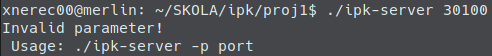
\includegraphics[scale=0.5]{1.png}\\\\
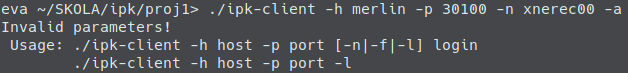
\includegraphics[scale=0.5]{3.png}\\\\
Spustenie serveru:\\
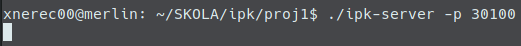
\includegraphics[scale=0.5]{2.png}\\\\
Spustenie klienta s parametrom -n:\\
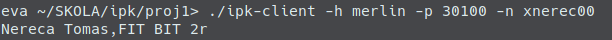
\includegraphics[scale=0.5]{4.png}\\\\
Spustenie klienta s parametrom -f:\\
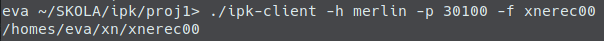
\includegraphics[scale=0.5]{5.png}\\\\
Spustenie klienta s parametrom -l a prefixom:\\
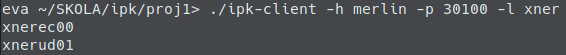
\includegraphics[scale=0.5]{6.png}\\\\
Spustenie klienta s parametrom -l bez prefixu (na obrázku len niekoľko riadkov):\\
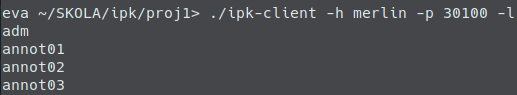
\includegraphics[scale=0.5]{7.png}

\section{Zdroje}
Pri riešení projektu som sa snažil čo najviac držať materiálov k predmetu. Pri návrhu TCP komunikácie som využil úryvky kódu z prednášky 2. 

Niektoré úryvky kódu sú inšpirované odpoveďami na diskusných fórach. Adresa na fórum je v tom prípade v komentári.

Ďalej som čerpal z rôznych manuálových stránok, napr.:

\url{http://man7.org/linux/}

\url{https://linux.die.net/man/}

\url{http://www.cplusplus.com/reference/}

\end{document}

